\makesectionpage[figures/quiz.png]{Klassifikation}

\makesubsectionpage{Grundidee}

\begin{frame}{Unsere Klassifikationsaufgabe}
\footnotesize
\begin{columns}
\column{0.35\textwidth}
Wir möchten einen \textbf{Kunststoff-Spritzgießprozess} überwachen.

\vspace{0.4em}
\begin{itemize}
  \item Für jeden \textbf{Fertigungszyklus} erfassen wir sensorisch die
        relevanten \textbf{Prozessgrößen}.
  \item Anhand dieser Prozessgrößen ziehen wir Rückschlüsse, ob im Zyklus
        ein \textbf{Gutteil} oder \textbf{Ausschuss} produziert wurde.
\end{itemize}

\vspace{0.4em}
{\footnotesize\itshape Zwei Klassen: Gutteil vs. Ausschuss --
binäre Klassifikation.}

\column{0.6\textwidth}
\centering
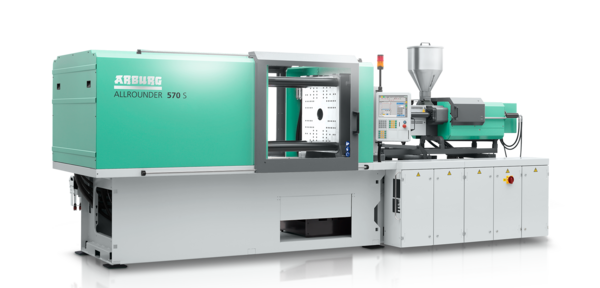
\includegraphics[width=\linewidth]{figures/arburg.png}
\end{columns}
\source{Bildquelle: \cite{arburg_allrounder520s}}
\end{frame}

\begin{frame}{Datenerfassung}
\begin{columns}
\column{0.60\textwidth}
\centering
\tiny
\includesvg[width=\linewidth]{figures/prinzip_spritzguss}

\column{0.35\textwidth}
Vermutung: Aus \textbf{maximalem Einspritzdruck} und der \textbf{Temperatur
am Fließweg-Ende} lässt sich erkennen, ob ein Zyklus erfolgreich war.

\vspace{0.5em}
\begin{itemize}
  \item Erfassung dieser Daten für \textbf{300 Spritzgießzyklen}.
  \item Manuelle Begutachtung der Teile.
  \item Klassifikation als \textbf{Gutteil} oder \textbf{Schlechtteil}.
\end{itemize}
\end{columns}
\source{Bildquelle: \cite{kaupp2014verfahren}}
\end{frame}


\begin{frame}{Unsere Klassifikationsaufgabe}
\begin{columns}
\column{0.47\textwidth}
Der Datensatz \texttt{qualitaet\_spritzguss.csv} hat folgende Struktur:

\vspace{0.6em}
\centering
{\footnotesize
\renewcommand{\arraystretch}{1.3}
\setlength{\tabcolsep}{6pt}
\begin{tabular}{r r r c}
& \textbf{Druck} & \textbf{Temperatur} & \textbf{Erfolg}\\
\hline
0 & 724.412449 & 226.006619 & 0\\
1 & 716.099585 & 225.297905 & 0\\
2 & 792.625755 & 234.443889 & 0\\
3 & 594.515152 & 231.452907 & 1\\
4 & 653.436610 & 224.344378 & 0\\
\end{tabular}}

\column{0.48\textwidth}
Die  Datensätze sind wie folgt verteilt:
\vspace{0.4em}
\centering
\includesvg[width=\linewidth]{figures/scatterplot_spritzguss_legende.svg}
\end{columns}
\end{frame}

\begin{frame}[fragile]{Visualisierung der Klassen}
\begin{columns}
\column{0.47\textwidth}

Die farbliche Unterscheidung der Klassen erreicht man mit dem Parameter
\texttt{c}.


\begin{minted}[fontsize=\footnotesize]{python}
%matplotlib inline
import matplotlib.pyplot as plt
plt.set_cmap("bwr")
plt.scatter(df["Druck"], df["Temperatur"],
            c=df["Erfolg"])
plt.xlabel("Druck [bar]")
plt.ylabel("Temperatur [°C]")
plt.show()
\end{minted}

\column{0.48\textwidth}
\centering
\includesvg[width=\linewidth]{figures/scatterplot_spritzguss}
\end{columns}
\source{Klassifikationstemplate.ipynb}
\end{frame}

\makesubsectionpage{Entscheidungsbäume}

\begin{frame}{Entscheidungsbäume: Grundidee}
\begin{columns}
\column{0.60\textwidth}
Wir spielen \textbf{„Wer bin ich?"}: Ein Spieler bekommt den Namen einer
bekannten Person auf die Stirn geklebt und kann ihn selbst nicht sehen.

\vspace{0.4em}
\begin{itemize}
  \item Ziel: die Person mit \textbf{möglichst wenigen Fragen} erraten.
  \item Vor der ersten Frage ist die Möglichkeitsmenge maximal.
  \item Jede Frage soll die Anzahl der Möglichkeiten \textbf{stark
        reduzieren}.
  \item[$\Rightarrow$] Die Frage nach dem Geschlecht \textbf{halbiert} die
        Ergebnismenge.
\end{itemize}

\column{0.35\textwidth}
\centering
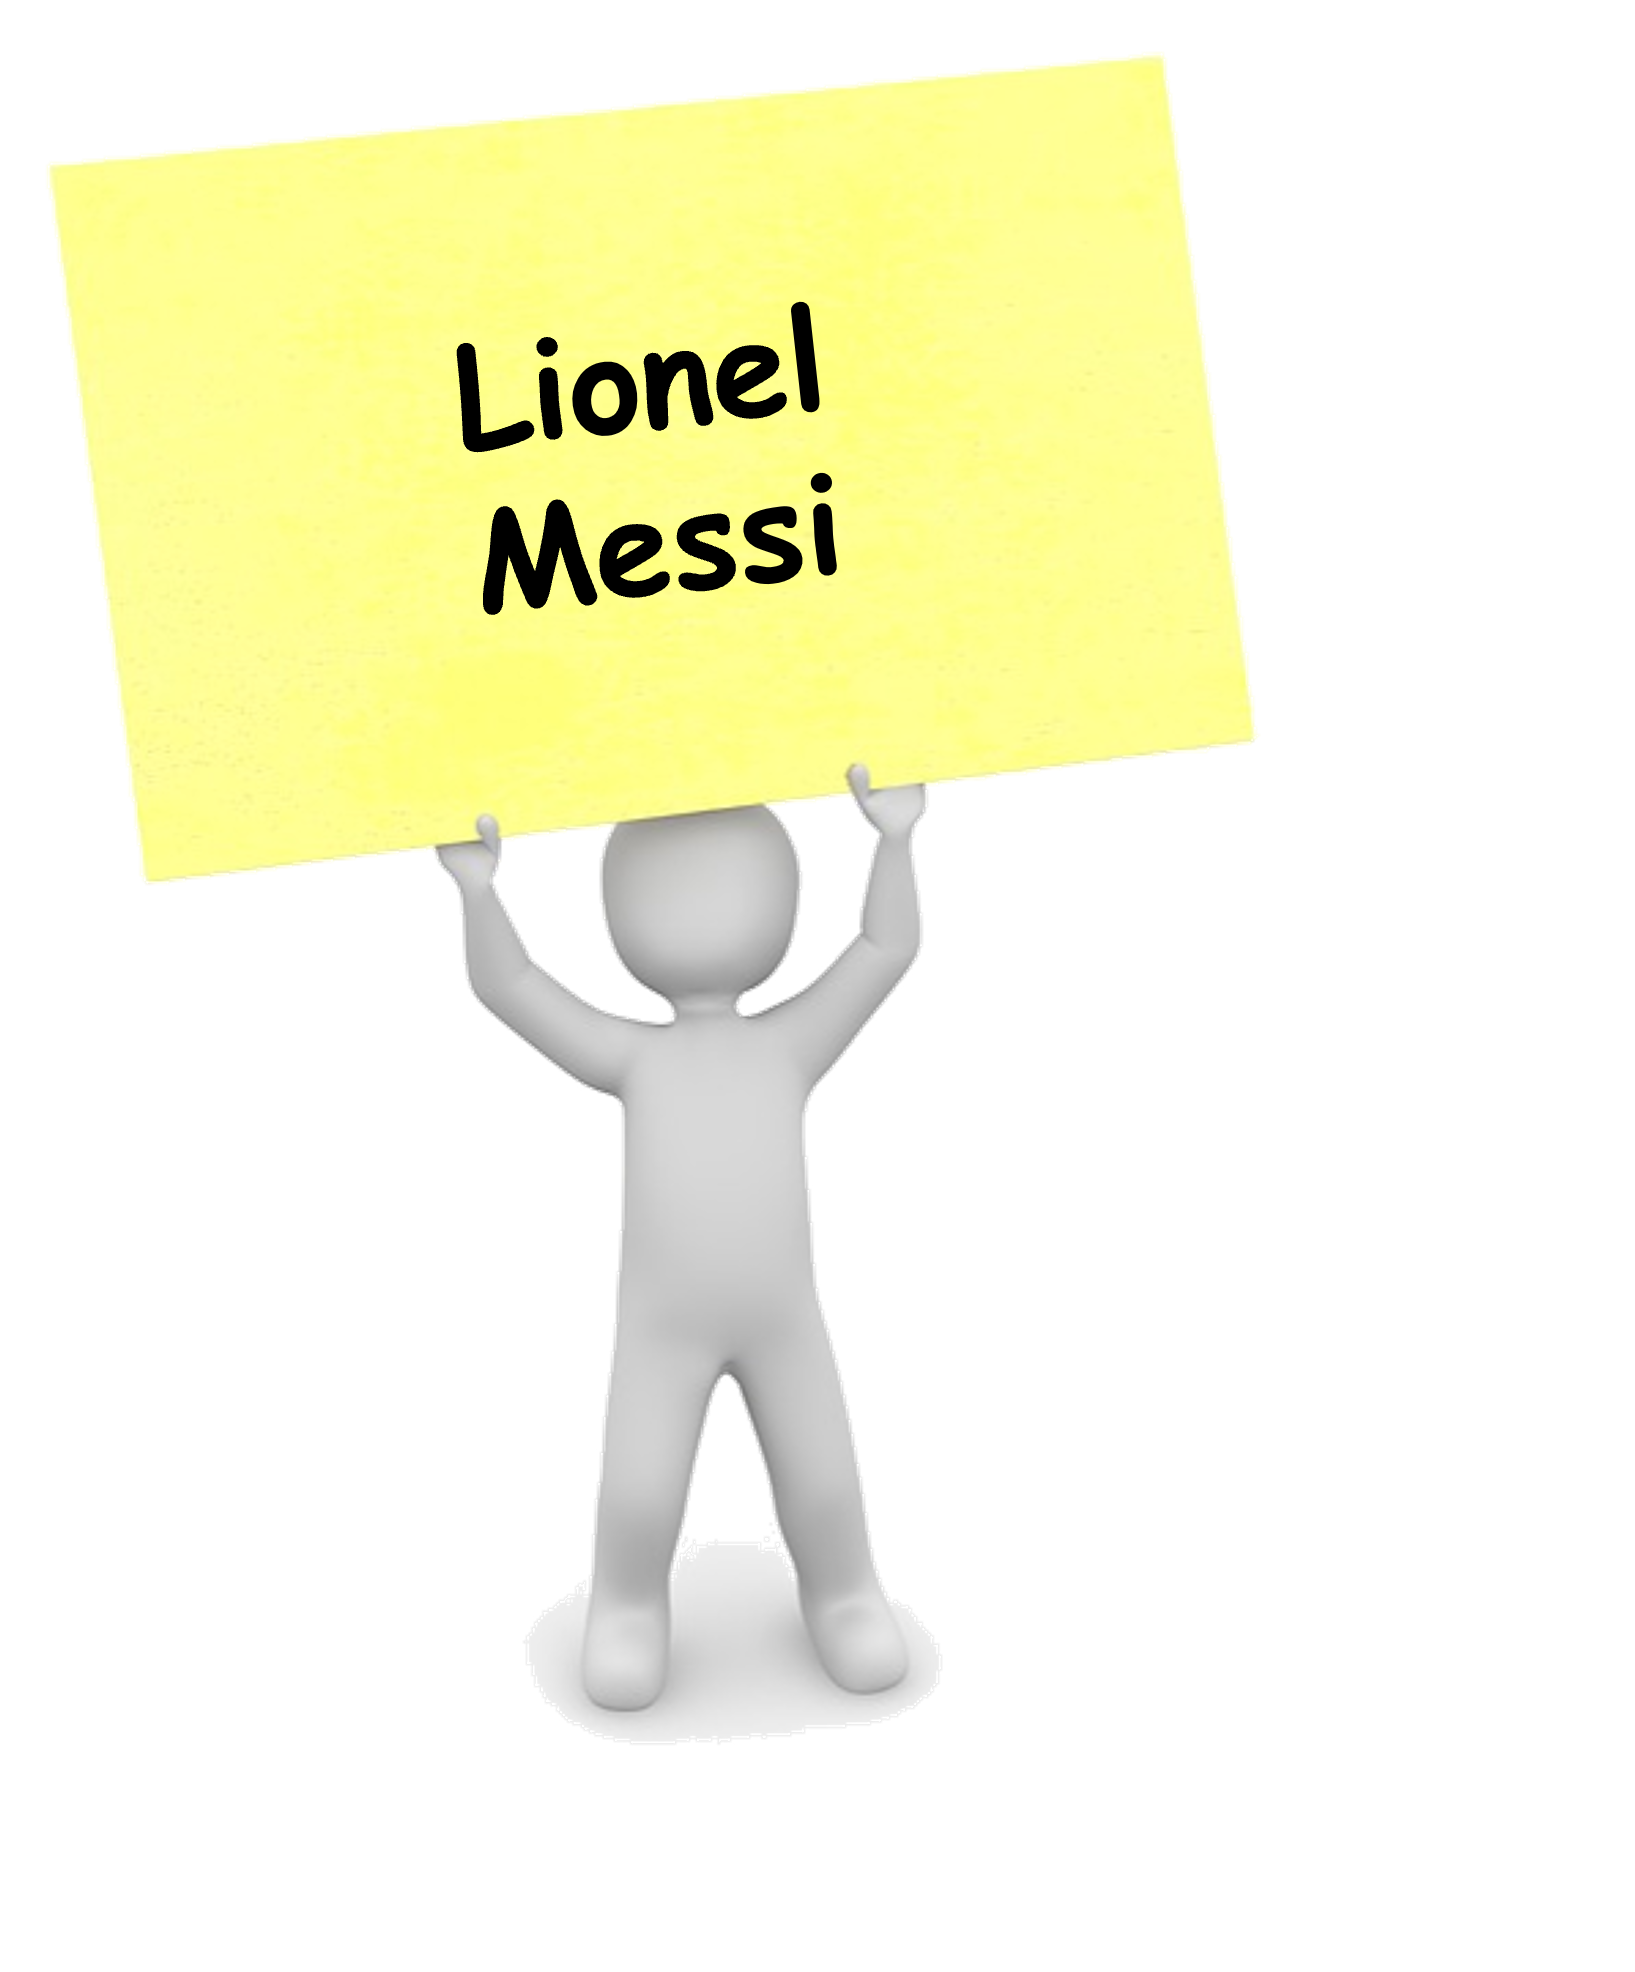
\includegraphics[width=\linewidth]{figures/WerBinIch.png}
\end{columns}
\source{\cite{seemann2024mlaz}}
\end{frame}


\begin{frame}{Entscheidungsbäume: Beispielbaum}
\begin{columns}
\column{0.60\textwidth}
\centering
\resizebox{\linewidth}{!}{%
\begin{tikzpicture}[
  frage/.style={draw=PrimaryColor, very thick, rounded corners=6pt,
                align=center, inner sep=6pt, text width=2.6cm,
                font=\footnotesize},
  raten/.style={draw=AccentTitle, very thick, rounded corners=6pt,
                align=center, inner sep=6pt, text width=2.4cm,
                font=\footnotesize},
  gefunden/.style={draw=ExampleTitle, very thick, rounded corners=6pt,
                align=center, inner sep=6pt, text width=2.4cm,
                font=\footnotesize\bfseries},
  kante/.style={->, >=Stealth, thick},
  lab/.style={font=\footnotesize, fill=white, inner sep=1pt}
]

\node[frage]    (q1)  at (0,0)        {Bin ich weiblich?};
\node[raten]    (r1)  at (-3.6,-2.1)  {Weiter raten\dots};
\node[frage]    (q2)  at (3.6,-2.1)   {Spiele ich Fußball?};
\node[frage]    (q3)  at (1.8,-4.4)   {Bin ich Lionel Messi?};
\node[raten]    (r2)  at (6.2,-4.4)   {Weiter raten\dots};
\node[gefunden] (g)   at (-0.2,-6.7)  {Gefunden!};
\node[raten]    (r3)  at (3.8,-6.7)   {Weiter raten\dots};

\draw[kante] (q1) -- (r1) node[lab, midway] {ja};
\draw[kante] (q1) -- (q2) node[lab, midway] {nein};
\draw[kante] (q2) -- (q3) node[lab, midway] {ja};
\draw[kante] (q2) -- (r2) node[lab, midway] {nein};
\draw[kante] (q3) -- (g)  node[lab, midway] {ja};
\draw[kante] (q3) -- (r3) node[lab, midway] {nein};

\end{tikzpicture}}

\column{0.35\textwidth}
\centering
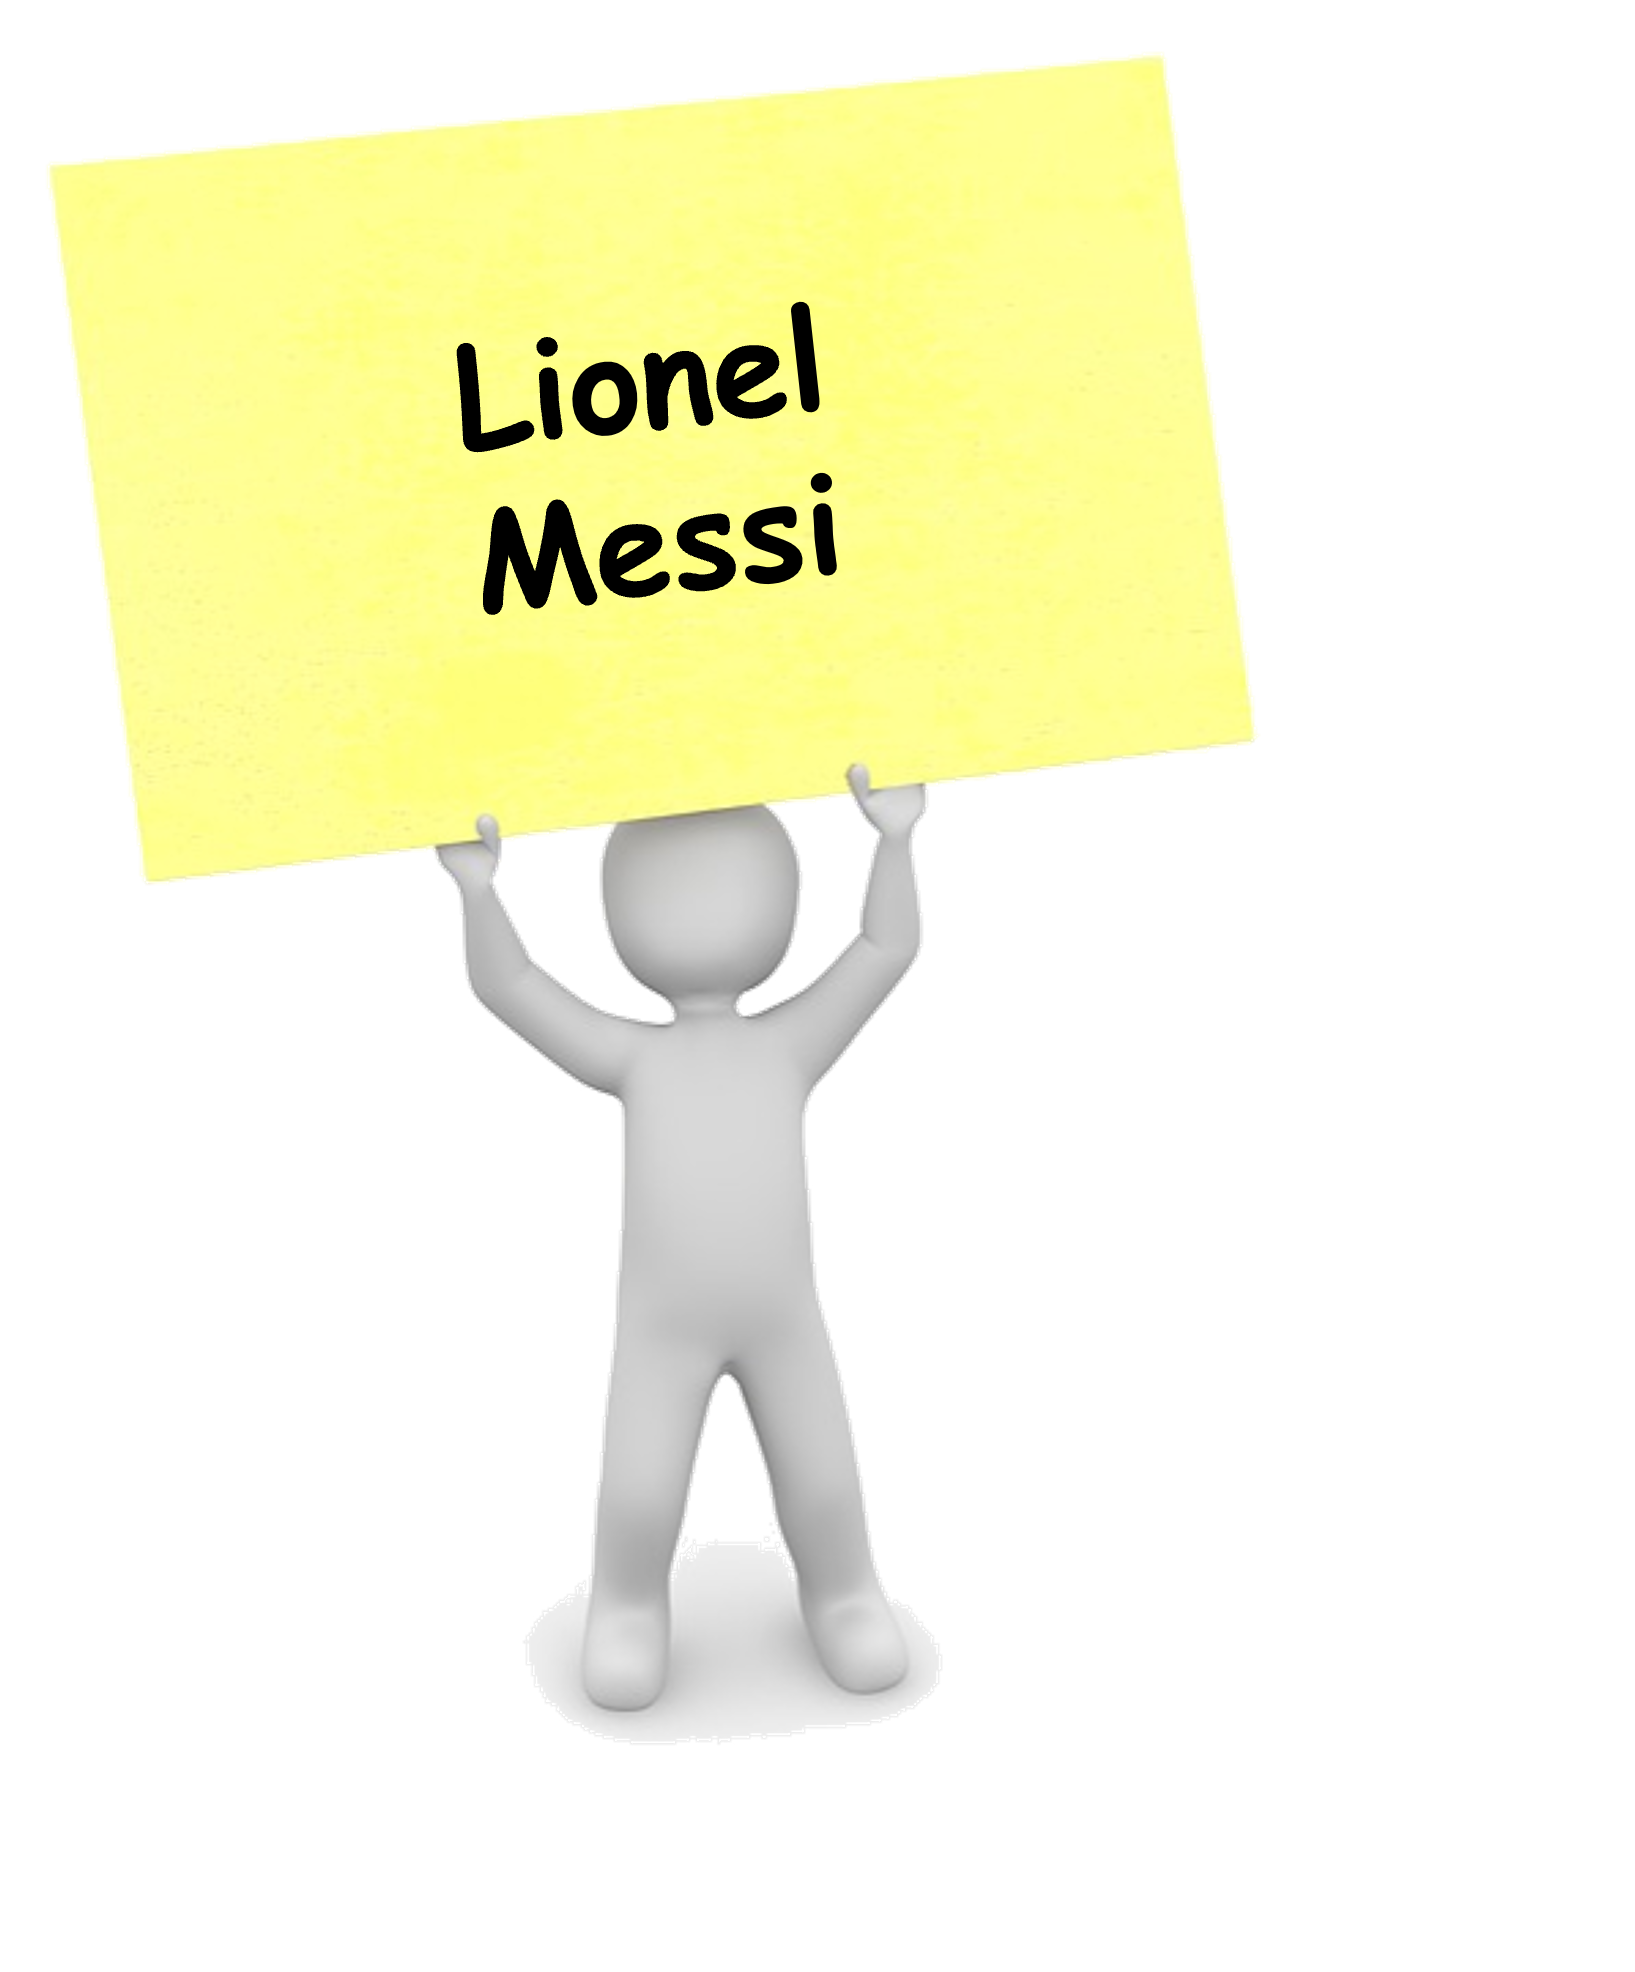
\includegraphics[width=\linewidth]{figures/WerBinIch.png}
\end{columns}
\source{\cite{seemann2024mlaz}}
\end{frame}

\begin{frame}{Entscheidungsbäume: Grundidee}
\begin{columns}
\column{0.47\textwidth}
Bei „Wer bin ich?" liegt ein \textbf{Spezialfall} vor: Jede Klasse kommt
nur einmal vor -- also rund \textbf{8,3 Mrd. Klassen}.

\vspace{0.4em}
\begin{itemize}
  \item Meist hat man nur \textbf{wenige Klassen}.
  \item Spritzgieß-Beispiel: zwei Klassen -- \textbf{gut} und
        \textbf{schlecht}.
  \item[$\Rightarrow$] Ziel: ein Entscheidungsbaum, der bisher
        \textbf{unbekannte} Zyklen beurteilt.
\end{itemize}

\column{0.48\textwidth}
\centering
\includesvg[width=\linewidth]{figures/scatterplot_spritzguss.svg}
\end{columns}
\end{frame}

\begin{frame}{Entscheidungsbäume: Grundidee}
\begin{columns}
\column{0.35\textwidth}
\centering
\includesvg[width=\linewidth]{figures/scatterplot_spritzguss.svg}

\column{0.60\textwidth}
\centering
Der resultierende Baum könnte etwa so aussehen:

\vspace{0.4em}
\resizebox{\linewidth}{!}{%
\begin{tikzpicture}[
  test/.style={draw=PrimaryColor, very thick, rounded corners=4pt,
               align=center, inner sep=6pt, text width=2.4cm,
               font=\footnotesize},
  gut/.style={draw=red, very thick, ellipse,
              align=center, inner sep=4pt, minimum width=1.8cm,
              font=\footnotesize},
  schlecht/.style={draw=blue, very thick, ellipse,
                   align=center, inner sep=4pt, minimum width=1.8cm,
                   font=\footnotesize},
  kante/.style={->, >=Stealth, thick},
  lab/.style={font=\footnotesize\itshape, fill=white, inner sep=1pt}
]

\node[test]     (d)  at (0,0)        {Druck < 800};
\node[test]     (t)  at (-2.4,-2.2)  {Temperatur < 250};
\node[gut]      (g1) at (2.6,-2.2)   {gut};
\node[schlecht] (s)  at (-4.0,-4.4)  {schlecht};
\node[gut]      (g2) at (-0.8,-4.4)  {gut};

\draw[kante] (d) -- (t)  node[lab, midway] {ja};
\draw[kante] (d) -- (g1) node[lab, midway] {nein};
\draw[kante] (t) -- (s)  node[lab, midway] {ja};
\draw[kante] (t) -- (g2) node[lab, midway] {nein};

\end{tikzpicture}}
\end{columns}
\source{\cite{seemann2024mlaz}}
\end{frame}


\begin{frame}{Entscheidungsbäume aus Trainingsdaten erstellen}
\begin{columns}
\column{0.60\textwidth}
Sollen Entscheidungsbäume für das \textbf{überwachte Lernen} eingesetzt
werden, braucht es Verfahren, die solche Bäume aus \textbf{Trainingsdaten
automatisch erstellen}.

\vspace{0.5em}
\begin{itemize}
  \item Eingabe: klassifizierte Trainingsdaten.
  \item Ausgabe: ein automatisch konstruierter Entscheidungsbaum.
  \item[$\Rightarrow$] Der Baum dient anschließend zur
        \textbf{Klassifikation} neuer Daten.
\end{itemize}

\column{0.35\textwidth}
\centering
\twemoji[width=0.9\linewidth]{deciduous tree}
\end{columns}
\source{\cite{seemann2024mlaz}}
\end{frame}

\begin{frame}{Entscheidungsbäume aus Trainingsdaten erstellen}
\begin{columns}
\column{0.47\textwidth}
\footnotesize
An jedem \textbf{Entscheidungsknoten} kommt eine Menge von Daten an.
\begin{itemize}
  \item Der Knoten teilt die Menge in \textbf{zwei Teilmengen}.
  \item Daten, die die Bedingung erfüllen zandern zum \textbf{ja}-Knoten.
  \item Alle übrigen $\rightarrow$ \textbf{nein}-Knoten.
\end{itemize}

\vspace{0.6em}
\centering
\begin{tikzpicture}[
  test/.style={draw=PrimaryColor, very thick, rounded corners=4pt,
               align=center, inner sep=6pt, text width=2.2cm,
               font=\footnotesize},
  kante/.style={->, >=Stealth, thick},
  lab/.style={font=\footnotesize\itshape, fill=white, inner sep=1pt}
]

\node[test] (d)  at (0,0)        {Druck < 800};
\coordinate (ja)   at (-2.,-1.5);
\coordinate (nein) at (2.,-1.5);

\draw[kante] (d) -- (ja)   node[lab, midway] {ja};
\draw[kante] (d) -- (nein) node[lab, midway] {nein};

\end{tikzpicture}

\column{0.48\textwidth}
\centering
\begin{tikzpicture}
  % SVG als Knoten platzieren
  \node[inner sep=0pt] (plot) at (0,0)
    {\includesvg[width=\linewidth]{figures/scatterplot_spritzguss.svg}};

  % senkrechter Strich bei Druck = 800
  % x-Position relativ zur Plotbreite justieren (hier ca. 60 %)
  \coordinate (xpos) at ($(plot.south west)!0.72!(plot.south east)$);
  \draw[ExampleTitle, very thick, dashed]
    (xpos) -- ($(plot.north west)!0.72!(plot.north east)$);
  
\end{tikzpicture}
\end{columns}
\source{\cite{seemann2024mlaz}}
\end{frame}

\begin{frame}{Entscheidungsbäume aus Trainingsdaten erstellen}
\begin{columns}
\column{0.40\textwidth}
Jede Entscheidung legt im Eingangsraum eine \textbf{Trenn-(hyper-)ebene}
fest.

\vspace{0.4em}
\begin{itemize}
  \item Im 2D-Raum: \textbf{senkrechte} oder \textbf{waagerechte} Geraden.
  \item Jede Gerade schneidet den Eingangsraum in \textbf{zwei Teile}.
\end{itemize}

\column{0.55\textwidth}
\centering
\resizebox{\linewidth}{!}{%
\begin{tikzpicture}[
  punkt/.style={circle, thick, minimum size=6pt, inner sep=0pt},
  schlecht/.style={punkt, fill=AccentColor, draw=AccentTitle},
  gut/.style={punkt, fill=PrimaryColor, draw=PrimaryTitle}
]

% Achsen mit dreieckigen Pfeilspitzen
\draw[-{Triangle[]}, thick] (0,0) -- (9,0)
  node[below, font=\small, pos=1, anchor=north east] {Druck [bar]};
\draw[-{Triangle[]}, thick] (0,0) -- (0,6)
  node[font=\small, rotate=90, anchor=south east, pos=1] {Temperatur [°C]};

% Trennebene bei Temperatur = 250
\draw[ExampleTitle, line width=2pt] (0,3) -- (8.6,3);
\node[font=\small] at (-0.4,3) {250};
\node[ExampleTitle, font=\small\itshape, anchor=west] at (7.6,3.6) {Trennebene};

% Schlechtteile
\node[schlecht] at (1.3,1.8) {};
\node[schlecht] at (2.6,1.4) {};
\node[schlecht] at (3.4,1.9) {};
\node[schlecht] at (2.4,2.6) {};
\node[schlecht] at (1.9,3.1) {};
\node[schlecht] at (3.4,3.1) {};
\node[schlecht] at (3.1,4.2) {};

% Gutteile
\node[gut] at (5.3,3.4) {};
\node[gut] at (5.8,2.7) {};
\node[gut] at (6.6,1.6) {};
\node[gut] at (5.5,1.3) {};
\node[gut] at (6.3,0.7) {};
\node[gut] at (7.0,2.5) {};
\node[gut] at (6.6,3.7) {};
\node[gut] at (5.9,4.6) {};
\node[gut] at (7.0,5.0) {};

\end{tikzpicture}}
\end{columns}
\source{\cite{seemann2024mlaz}}
\end{frame}

\begin{frame}{Entscheidungsbäume aus Trainingsdaten erstellen}
\begin{columns}
\column{0.40\textwidth}
Die Lernverfahren versuchen, die \textbf{Trennebenen} (durch geeignete
Bedingungen) so zu legen, dass die entstehenden Teilmengen möglichst
\textbf{homogen} bezüglich der Zielklasse sind.

\begin{itemize}
  \item Idealerweise enthält jede Teilmenge nur Datensätze \textbf{derselben
        Klasse}.
\end{itemize}

\column{0.55\textwidth}
\centering
\resizebox{\linewidth}{!}{%
\begin{tikzpicture}[
  punkt/.style={circle, thick, minimum size=6pt, inner sep=0pt},
  schlecht/.style={punkt, fill=AccentColor, draw=AccentTitle},
  gut/.style={punkt, fill=PrimaryColor, draw=PrimaryTitle}
]

% Achsen mit dreieckigen Pfeilspitzen
\draw[-{Triangle[]}, thick] (0,0) -- (9,0)
  node[below, font=\small, pos=1, anchor=north east] {Druck [bar]};
\draw[-{Triangle[]}, thick] (0,0) -- (0,6)
  node[font=\small, rotate=90, anchor=south east, pos=1] {Temperatur [°C]};

% Trennebene bei Druck = 800 (senkrecht)
\draw[ExampleTitle, line width=2pt] (4.3,0) -- (4.3,5.6);
\draw[ExampleTitle, thick] (4.3,0.12) -- (4.3,-0.12);
\node[font=\small, anchor=north] at (4.3,-0.15) {800};
\node[ExampleTitle, font=\small\itshape, anchor=south] at (4.3,5.6) {Trennebene};

% Schlechtteile
\node[schlecht] at (1.3,1.8) {};
\node[schlecht] at (2.6,1.4) {};
\node[schlecht] at (3.4,1.9) {};
\node[schlecht] at (2.4,2.6) {};
\node[schlecht] at (1.9,3.1) {};
\node[schlecht] at (3.4,3.1) {};
\node[schlecht] at (3.1,4.2) {};

% Gutteile
\node[gut] at (5.3,3.4) {};
\node[gut] at (5.8,2.7) {};
\node[gut] at (6.6,1.6) {};
\node[gut] at (5.5,1.3) {};
\node[gut] at (6.3,0.7) {};
\node[gut] at (7.0,2.5) {};
\node[gut] at (6.6,3.7) {};
\node[gut] at (5.9,4.6) {};
\node[gut] at (7.0,5.0) {};

\end{tikzpicture}}
\end{columns}
\source{\cite{seemann2024mlaz}}
\end{frame}

\begin{frame}{Entscheidungsbäume aus Trainingsdaten erstellen}
\begin{columns}
\column{0.47\textwidth}
\footnotesize
\begin{itemize}
  \item In der Regel gelingt es nicht, die Daten schon im \textbf{ersten Schritt}
komplett „klassenrein" aufzuteilen.
  \item Durch jede weitere Abfrage versucht man, die \textbf{Homogenität} zu
        erhöhen.
\end{itemize}

\vspace{0.4em}
\centering
\resizebox{0.8\linewidth}{!}{%
\begin{tikzpicture}[
  test/.style={draw=PrimaryColor, very thick, rounded corners=4pt,
               align=center, inner sep=6pt, text width=2.4cm,
               font=\footnotesize},
  gut/.style={draw=PrimaryTitle, very thick, ellipse,
              align=center, inner sep=4pt, minimum width=1.8cm,
              font=\footnotesize},
  schlecht/.style={draw=AccentTitle, very thick, ellipse,
                   align=center, inner sep=4pt, minimum width=1.8cm,
                   font=\footnotesize},
  kante/.style={->, >=Stealth, thick},
  lab/.style={font=\footnotesize\itshape, fill=white, inner sep=1pt}
]

\node[test]     (d)  at (0,0)        {Druck < 800};
\node[test]     (t)  at (-2.4,-2.2)  {Temperatur < 250};
\node[gut]      (g1) at (2.6,-2.2)   {gut};
\node[schlecht] (s)  at (-4.0,-4.4)  {schlecht};
\node[gut]      (g2) at (-0.8,-4.4)  {gut};

\draw[kante] (d) -- (t)  node[lab, midway] {ja};
\draw[kante] (d) -- (g1) node[lab, midway] {nein};
\draw[kante] (t) -- (s)  node[lab, midway] {ja};
\draw[kante] (t) -- (g2) node[lab, midway] {nein};

\end{tikzpicture}}

\column{0.48\textwidth}
\centering
\resizebox{\linewidth}{!}{%
\begin{tikzpicture}[
  punkt/.style={circle, thick, minimum size=6pt, inner sep=0pt},
  schlecht/.style={punkt, fill=AccentColor, draw=AccentTitle},
  gut/.style={punkt, fill=PrimaryColor, draw=PrimaryTitle}
]

% Achsen mit dreieckigen Pfeilspitzen
\draw[-{Triangle[]}, thick] (0,0) -- (7.5,0)
  node[below, font=\small, pos=1, anchor=north east] {Druck [bar]};
\draw[-{Triangle[]}, thick] (0,0) -- (0,6)
  node[font=\small, rotate=90, anchor=south east, pos=1] {Temperatur [°C]};

% Trennebene 1: senkrecht bei Druck = 800
\draw[ExampleTitle, line width=2pt] (4.3,0) -- (4.3,5.8);
\draw[ExampleTitle, thick] (4.3,0.12) -- (4.3,-0.12);
\node[font=\small, anchor=north] at (4.3,-0.15) {800};
\node[ExampleTitle, font=\small\itshape, anchor=south west] at (4.6,5.6) {Trennebene 1};

% Trennebene 2: waagerecht (nur links von 800) bei Temperatur = 250
\draw[ExampleTitle, line width=2pt] (0,4.0) -- (4.3,4.0);
\node[ExampleTitle, font=\small\itshape, anchor=north west] at (0.3,3.8) {Trennebene 2};

% Schlechtteile (unten links)
\node[schlecht] at (2.8,3.5) {};
\node[schlecht] at (1.5,2.9) {};
\node[schlecht] at (3.0,2.9) {};
\node[schlecht] at (2.3,2.4) {};
\node[schlecht] at (1.0,1.5) {};
\node[schlecht] at (2.8,1.5) {};
\node[schlecht] at (2.0,1.0) {};

% Gutteile oben links (ueber Trennebene 2)
\node[gut] at (0.8,4.5) {};
\node[gut] at (1.5,5.4) {};
\node[gut] at (2.5,5.7) {};
\node[gut] at (2.3,4.9) {};

% Gutteile rechts (ueber Trennebene 1)
\node[gut] at (5.3,4.4) {};
\node[gut] at (5.0,3.2) {};
\node[gut] at (6.0,3.0) {};
\node[gut] at (5.5,2.2) {};
\node[gut] at (6.0,1.5) {};
\node[gut] at (5.0,1.0) {};
\node[gut] at (5.8,0.6) {};

\end{tikzpicture}}
\end{columns}
\source{\cite{seemann2024mlaz}}
\end{frame}


\begin{frame}{Entscheidungsbäume aus Trainingsdaten erstellen}
\begin{columns}
\column{0.35\textwidth}
\centering
\twemoji[width=0.9\linewidth]{balance scale}

\column{0.60\textwidth}
Jeder Knoten teilt die ankommende Datenmenge in \textbf{zwei disjunkte
Teilmengen}. Ein Entscheidungsbaum entsteht, indem solche Knoten verbunden
werden.

\vspace{0.4em}
\textbf{Wann ist ein Baum „gut"?} Ein guter Entscheidungsbaum
\begin{itemize}
  \item macht \textbf{möglichst wenige Fehler} und
  \item ist -- unter den fehlerärmsten Bäumen -- der \textbf{kleinste}, der
        eine gültige Entscheidung liefert.
\end{itemize}

\vspace{0.4em}
{\footnotesize\itshape Größenmaße: Baumhöhe, Anzahl der Blätter oder
Pfadlängensumme.}
\end{columns}
\source{\cite{Frochte2020}}
\end{frame}

\begin{frame}{Wie findet man einen kleinen, genauen Baum?}
\begin{columns}
\column{0.47\textwidth}
\begin{blockC1}{Optimalen Baum finden}
\begin{itemize}
  \item Problem ist \textbf{NP-vollständig}.
  \item Rechnerisch herausfordernd.
  \item Liefert potenziell die \textbf{genaueste} Lösung.
\end{itemize}
\end{blockC1}

\column{0.48\textwidth}
\begin{blockC2}{Heuristiken verwenden}
\begin{itemize}
  \item Liefert \textbf{praktikable}, aber nicht perfekte Lösungen.
  \item Besonders wichtig bei \textbf{größeren Datenmengen}.
\end{itemize}
\end{blockC2}
\end{columns}

\vspace{0.6em}
\centering
{\footnotesize\itshape In der Praxis nutzt man daher fast immer Heuristiken.}
\source{\cite{Frochte2020}}
\end{frame}


\begin{frame}{ID3-Algorithmus}
\begin{columns}
\column{0.65\textwidth}
\textbf{ID3} (Iterative Dichotomiser 3)
\begin{itemize}
  \item Entwickelt von \textbf{Ross Quinlan} in den 1980er Jahren.
  \item Einfache Struktur -- ideal als \textbf{Einstiegsbeispiel}.
  \item Fokus: Klassifikation mit \textbf{nominalen Merkmalen}.
\end{itemize}

\vspace{0.4em}
\begin{blockC1}{Eigenschaften}
\begin{itemize}
  \item Effizient bei vielen Features.
  \item Erzeugt vergleichsweise \textbf{einfache} Bäume.
  \item \textbf{Keine Garantie} für optimale Bäume.
\end{itemize}
\end{blockC1}

\column{0.3\textwidth}
\begin{blockDef}{Dichotomiser}
Verfahren zur \textbf{schrittweisen Aufspaltung} von Daten in Teilgruppen
zur Erstellung eines Entscheidungsbaums.
\end{blockDef}
\end{columns}
\source{\cite{Frochte2020}}
\end{frame}

\begin{frame}{ID3-Algorithmus: Beispieldatensatz}
\begin{columns}
    \footnotesize
\column{0.3\textwidth}
Entscheidungsbäume basieren auf einem gegebenen \textbf{Datenbestand}.

\begin{itemize}
  \item ID3: Fokus auf \textbf{nominalskalierte} Merkmale.
  \item Ziel: Klassifikation anhand \textbf{diskreter} Werte.
\end{itemize}

\vspace{0.4em}
{\footnotesize\itshape Beispiel: tägliches Protokoll, ob jemand mit dem Rad
zur Arbeit fährt.}

\column{0.65\textwidth}
\centering
{\scriptsize
\renewcommand{\arraystretch}{1.3}
\setlength{\tabcolsep}{4pt}
\rowcolors{2}{SecondaryColor!12}{white}
\begin{tabular}{c l c c c c c}
\rowcolor{PrimaryColor}
\textcolor{white}{\textbf{Nr.}} &
\textcolor{white}{\textbf{Wetter}} &
\textcolor{white}{\textbf{Sonnig?}} &
\textcolor{white}{\textbf{Schnee}} &
\textcolor{white}{\textbf{Auto defekt}} &
\textcolor{white}{\textbf{Start 08:00}} &
\textcolor{white}{\textbf{Rad fahren}}\\
1 & sonnig & Ja   & Nein & Nein & Nein & Ja\\
2 & Regen  & Nein & Nein & Nein & Nein & Nein\\
3 & Regen  & Nein & Nein & Ja   & Nein & Ja\\
4 & Regen  & Nein & Nein & Nein & Nein & Nein\\
5 & sonnig & Ja   & Nein & Ja   & Nein & Ja\\
6 & Regen  & Nein & Nein & Ja   & Ja   & Ja\\
7 & sonnig & Ja   & Nein & Nein & Ja   & Nein\\
8 & sonnig & Ja   & Ja   & Nein & Nein & Nein\\
9 & sonnig & Ja   & Ja   & Ja   & Nein & Nein\\
\dots & \dots & \dots & \dots & \dots & \dots & \dots\\
\end{tabular}}
\end{columns}
\source{\cite{Frochte2020}}
\end{frame}

\begin{frame}{ID3-Algorithmus: Zielsetzung}
\begin{columns}
\column{0.3\textwidth}
\footnotesize
\textbf{Ziel:} Prognosesystem für „Radfahren zur Arbeit".

\vspace{0.4em}
\begin{itemize}
  \item Gegeben: Menge $X$ der Kenngrößen-Vektoren und Menge $Y$ der
        Ausgabewerte (Rad fahren: Ja/Nein).
  \item Datengrundlage: Trainingsdaten $D \subset X \times Y$.
  \item Ergebnis: ein \textbf{Entscheidungsbaum} wie rechts.
\end{itemize}

\column{0.65\textwidth}
\centering
\resizebox{\linewidth}{!}{%
\begin{tikzpicture}[
  test/.style={draw=PrimaryColor, very thick, rounded corners=4pt,
               align=center, inner sep=5pt, text width=1.9cm,
               font=\footnotesize},
  rad/.style={draw=ExampleTitle, very thick, ellipse,
              align=center, inner sep=2pt, text width=1.3cm,
              minimum height=1.3cm, font=\scriptsize},
  nicht/.style={draw=AlertTitle, very thick, ellipse,
                align=center, inner sep=2pt, text width=1.3cm,
                minimum height=1.3cm, font=\scriptsize},
  kante/.style={->, >=Stealth, thick},
  lab/.style={font=\footnotesize\itshape, fill=white, inner sep=1pt}
]

% Knoten
\node[test]  (w)   at (0,0)        {Wetterlage sonnig};
\node[test]  (sch) at (-4.0,-2.3)  {Schnee};
\node[test]  (auto)at (4.0,-2.3)   {Auto kaputt};
\node[nicht] (n1)  at (-6.0,-4.8)  {nicht\\Rad fahren};
\node[test]  (start)at (-2.6,-4.8) {Start 8 Uhr};
\node[rad]   (r1)  at (2.4,-4.8)   {Rad\\fahren};
\node[nicht] (n2)  at (5.6,-4.8)   {nicht\\Rad fahren};
\node[nicht] (n3)  at (-3.8,-7.3)  {nicht\\Rad fahren};
\node[rad]   (r2)  at (-1.4,-7.3)  {Rad\\fahren};

% Kanten
\draw[kante] (w) -- (sch)   node[lab, midway] {ja};
\draw[kante] (w) -- (auto)  node[lab, midway] {nein};
\draw[kante] (sch) -- (n1)  node[lab, midway] {ja};
\draw[kante] (sch) -- (start)node[lab, midway] {nein};
\draw[kante] (auto) -- (r1) node[lab, midway] {ja};
\draw[kante] (auto) -- (n2) node[lab, midway] {nein};
\draw[kante] (start) -- (n3)node[lab, midway] {ja};
\draw[kante] (start) -- (r2)node[lab, midway] {nein};

\end{tikzpicture}}
\end{columns}
\source{\cite{Frochte2020}}
\end{frame}

\begin{frame}{Algorithmus zur Entscheidungsbaumerzeugung}
\begin{columns}
\column{0.6\textwidth}
\scriptsize
\begin{algorithm}[H]
\SetAlgoCaptionLayout{scriptsize}
\KwIn{Beispielmenge $D$, Merkmale $A = \{A_1, \dots, A_n\}$}
\KwOut{Entscheidungsbaum}
\SetKwFunction{FMain}{GENTREE}
\SetKwProg{Fn}{Prozedur}{:}{}
\Fn{\FMain{$D$, $A$}}{
  \If{$D$ einklassig}{
    Blatt mit dieser Klasse\;
    \Return\;
  }
  \If{$A = \emptyset$}{
    Blatt mit Mehrheitsklasse\;
    \Return\;
  }
  Wähle $A_i \in A$ mit $r$ Werten\;
  Teile $D$ nach $A_i$ in $D_1, \dots, D_r$\;
  \ForEach{$D_j$}{
    \eIf{$D_j \neq \emptyset$}{
      \FMain{$D_j$, $A \setminus \{A_i\}$}\;
    }{
      Blatt mit Mehrheitsklasse\;
    }
  }
}
\caption{Entscheidungsbaum-Erzeugung}
\end{algorithm}

\column{0.35\textwidth}
\begin{itemize}
  \item Die konketen Verfahren unterscheiden sich nur in der \textbf{Merkmalsauswahl}.
  \item Der Grundalgorithmus erlaubt auch Prüfungen mit \textbf{mehr als zwei
        Ausgängen}.
  \item Wir arbeiten aber stets mit \textbf{Binärbäumen}.
  \item \textbf{Rekursiver Aufruf} für alle Teilmengen.
\end{itemize}
\end{columns}
\source{\cite{Frochte2020}}
\end{frame}

\makequizpage{\QUIZURL}{\QUIZQRCODE}{\QUIZIMAGE}
\makequestionspage{\FRAGENIMAGE}